
\section{\textit{Edge computing}}

У контексту \textit{Edge computing}-a, термин \textit{edge} се посебно односи на географску или логичку границу мреже где се обрада података одвија ближе извору података или уређају крајњег корисника, уместо да се ослања само на централизоване центре података или сервере у \textit{cloud}-у. Иако ова идеја постоји већ годинама уназад, оно што је условило њену тренутну популаризацију и  развој је долазак 5G мреже на тржиште која омогућава међусобну комуникацију много већег броја уређаја, као и много већи пропусни опсег без којих реализација овакве архитектуре не би била могућа.\\

Oсновне карактеристике \textit{edge comptuing}-a су:
\begin{itemize}
    \item Близина извора података. Уређаји који обрађују и анализирају податке налазе се веома близу самог извора података, тиме смањујући кашњење и побољшавајући време одговора за критичне апликације.

    \item Децентрализација. Ресурси за израчунавање и аналитику распоређују се преко \textit{edge} уређаја, сервера и \textit{gateway}-a омогућавајући локално процесирање података и одлучивање.
\end{itemize}

\subsection{Архитектура}

Aрхитектура оваквих система најчешће се састоји из три слоја \ref{fig:edge_arch}:

\begin{itemize}
    \item Слој крајњих уређаја, који се састоји од разних сензорских и мобилних уређаја као и уређаја који не морају само да прикупљају информације, него и да реагују у складу са наредбама система.

    \item \textit{Edge} слој који служи за горе поменуту обраду и анализу података у близини самих крајњих уређаја, која смањује латеницју и оптерећење на мрежи. Обрађујући податке на овом слоју, такође се повећава и безбедност система пошто прикупљени и обрађени подаци ни у једном тренутку не морају напустити интерну мрежу организације.

    \item \textit{Cloud} слој на који се шаљу задаци који превазилазе моћи {еdge} слоја, као и подаци који су намењени за глобалну употребу, који су додатно филтрирани и шифровани ради боље заштите података јер њиховим слањем на \textit{cloud} они су изложени свакаквим врстама напада који иначе нису могући у крајњим и \textit{еdge} слојевима.

\end{itemize}

\begin{figure}[H]
    \centering
    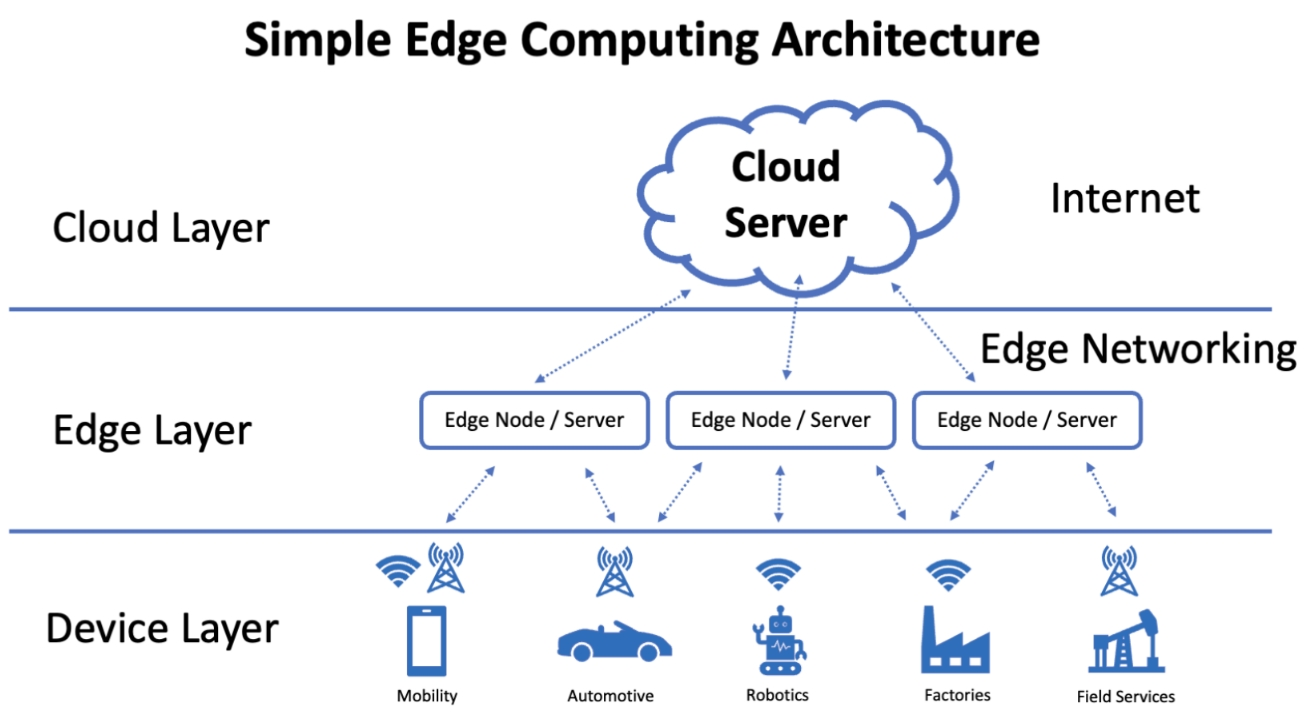
\includegraphics[width=1\textwidth]{images/edge_arch.jpg}
    \caption{Скица уобичајене \textit{edge} архитектуре}
    \label{fig:edge_arch}
\end{figure}

\subsection{Могуће примене}

Локалност, брзина и безбедност израчунавања \textit{edge computing}-a може бити од користи у разним случајевима:

    \subsubsection{Предикитвно одржавање машина у погонима} Неочекивани отказ машинa у индустријским погонима може значајно угрозити рад, профит фирме као и безбедност радника који њима управљају или се налазе у њиховој близини. Тренутни, најчешћи начин превеницје отказа оваквих машина обаваља се редовним, заказаним контролама и сервисима. Овакав приступ превенцији се показао као ефикасан, али његов проблем је што тешко и једино искуствено може одредити интервал између две контроле што резултује сувише честим или ретким контролама, што може довести до ненаданог престанка рада машине или узалудног губитка ресурса на сувишне контроле. \textit{Edge computing} овај проблем решава константим праћењем рада и стања сваке појединачне машине у реалном или приближно реалном времену помоћу мноштва сензора који су повезани или интегрисани у машине. На овај начин нема потребе за нагађањем времена контроле или поправке машине, због тога што се информације о стању машине могу добавити у било ком тренутку и по потреби организовати њихово сервисирање.

    \subsubsection{Видео надзор подржан вештачком интелигенцијом}

    Видео надзор је један од најраспрострањенијих начина константног удаљеног надзора, добављања информација, као и превенције нежељених догађаја. Све већим развојем вештачке интелигенције, могућности видео надзора се проширују са пуког посматрања снимака камера од стране човека на ауто детекцију објеката и препознавање значајних догађаја, попут уласка непознатих лица у објекат или присуства човека у деловима погона који могу угрозити његово здравље или живот. Оваква примена вештачке интелигенције захтева обраду података у реалном времену, као и конекцију са одређеним базама података и серверима који када би се налазили на \textit{cloud} платформама не би успевали да постигну најбоље перформансе и случајеви нестанка интернет конекције доводили би до потпуног отказа система. Због ових потешкоћа \textit{edge computing} је добар кандидат за имплементацију ових система због своје локалности уређаја за обраду података која смањује вероватноћу велике латенције и отказа комуникације између компоненти система.

    \subsubsection{Пренос догађаја уживо}

    Видео преноси утакмица, конференција и осталих догађаја временом добијају на квалитету што све више и више оптерећује њихов мрежни пренос. Закшњење које се јавља може представљати проблем гледаоцима који се налазе у непосредној близини самог догађаја. С тога се уместо слања на централни \textit{cloud} сервер, видео садржај поставља на локално распоређене \textit{edge} сервере којима гледаоци могу приступити са веома малом латенцијом. 